%Item 5
\chapter{Implementaci\'on (entrega y operaci\'on)}
\newpage
Para poder ocupar en forma correcta \emph{VIPeR} se va a necesitar:
\begin{itemize}
\item Un smartphone con sistema operativo Android versi\'on 2.1 o superior y que tenga al menos la posibilidad de ocupar bluetooth y pantalla t\'actil.
\item Un robot LEGO Mindstorms versi\'on NXT, con al menos:
  \begin{itemize}
  \item Dos bricks. 
  \item Seis motores
  \item Lista de sensores usados por nuestro robot
  \end{itemize}
\end{itemize}

%
%Item 5.1
%
\section{Plan de operaci\'on del sistema}
Los usuarios del producto ser\'an personas portadoras de Smartphones con Sistema Operativo Android, con \'enfasis en estudiantes de ense\~nanza media. 

Cuando un usuario use \emph{VIPeR} por primera vez va a tener la posibilidad de configurar en la aplicaci\'on su mascota de acuerdo a sus gustos (nombre, tipo de mascota). La pantalla de configuraci\'on incluye la calibraci\'on de los motores y sensores de acuerdo a una configuraci\'on predeterminada de robot. Si bien est\'a dise\~nado para interactuar con un robot LEGO Mindstorms, cabe destacar que ser\'a posible hacer uso de la aplicaci\'on sin necesidad de tener un robot real. En ese caso va a tener funcionalidad limitada a las funciones disponibles en el smartphone. Los usuarios tendr\'an acceso a indicaciones sobre la instalaci\'on y uso de \emph{VIPeR}.

Phyrex, como pre-empresa responsable del desarrollo de \emph{VIPeR}, se compromete de manera \'integra con los siguientes puntos respecto al sistema:
\begin{itemize}
\item Cumplimiento total de requerimientos en plazos acordados con el cliente
\item Producto orientado al usuario, interfaz intuitiva.
\item Asistencia t\'ecnica en el uso de la aplicaci\'on, la cual puede ser entregada por medio de la website oficial o Facebook.
\item Soluci\'on pronta de errores ocurridos en la aplicaci\'on.
\end{itemize}

\newpage
%
%Item 5.2
%
\section{Plan de implementaci\'on (entrega)}
La iniciativa se basa en un plan inicial de promoci\'on informativa del producto, el cual tiene 3 fases:

\begin{enumerate}
\item Reconocimiento del producto: Dar a conocer mediante website, redes sociales (Facebook, Twitter, Google+) presentando la empresa y explicando en qu\'e consiste a grandes rasgos nuestro producto. El objetivo principal es traer a potenciales usuarios y gente interesada que permita una mayor comunicaci\'on externa y genere una imagen general de nosotros y un posicionamiento inicial enfocado en la innovaci\'on.
\item Integraci\'on de potenciales usuarios: Actualizaciones peri\'odicas sobre el producto mediante anuncios y elementos audiovisuales los cuales se situar\'an en los medios usados en fase 1. El objetivo principal es interiorizar a los interesados no s\'olo en el producto final, sino que en su mejora posterior, dando oportunidad de opini\'on a los mismos usuarios sobre posibles caracter\'isticas incorporables en \'este.
\item Consolidaci\'on: Dejar accesible la aplicaci\'on en la website oficial y luego a trav\'es de Google Play de manera gratuita. El c\'odigo necesario para que el robot interact\'ue con el smartphone va a estar disponible en una descarga aparte, la cual estar\'a presente en la p\'agina oficial.
\end{enumerate}

Una vez disponible la aplicaci\'on, la instalaci\'on se puede realizar de manera independiente por los usuarios.

%
%Item 5.2.1
%
\newpage
\subsection{Diagramas de Casos de Uso}

%
%ENTREGABLE 1
%
\subsubsection{Entregable 1}

Los casos de uso correspondientes al Entregable 1 se detallan a continuaci\'on, desde la tabla~\ref{table:CrearMascota} hasta la tabla~\ref{table:CalibrarRobot}. En figura~\ref{fig:Caso1}, se muestra el diagrama de los casos de uso a implementar.

\begin{figure}[H]
  \centering
  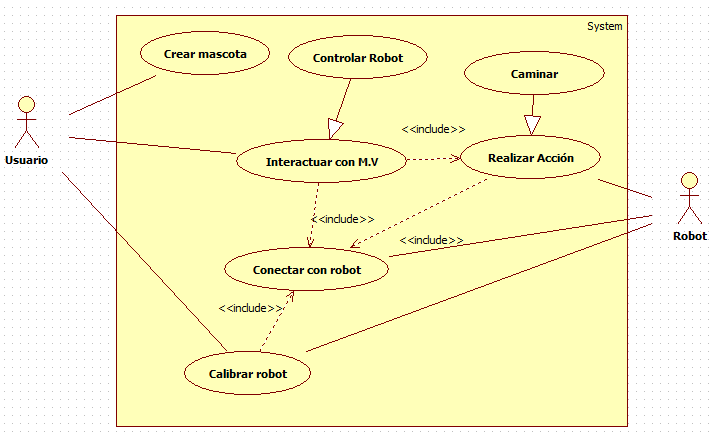
\includegraphics[scale=0.6]{caso1.png}
  \caption[~Caso de Uso Entregable 1]{Caso de Uso para el Entregable 1.}
  \label{fig:Caso1}
\end{figure}

%%
%%Caso de Uso: Crear Mascota
%%
\begin{table}[htbp!]
  \centering
  \begin{tabular}{|p{4cm}|p{6cm}|}\hline
    \bf{Caso de Uso}  & Crear Mascota. \\ \hline
    \bf{Descripci\'on} & Introducir datos generales de mascota (nombre, fecha de nacimiento --para calcular la edad--, raza, color, MAC --para conectar al robot--). \\ \hline
    \bf{Pre-condiciones} &  Que no haya mascota viva o creada. \\ \hline
    \bf{Post-condiciones} & Queda pareado el robot con el dispositivo Android, se ha creado una nueva mascota en la base de datos, se muestra la pantalla principal de la aplicaci\'on con la mascota creada. \\ \hline
    \bf{Requerimientos no funcionales} & Dispositivo Android con Bluetooth, robot LEGO Mindstorms encendido. \\ \hline
  \end{tabular}
  \caption[~Caso de Uso: Crear Mascota]{Caso de Uso: Crear Mascota.}
  \label{table:CrearMascota}
\end{table}

%%
%%Caso de Uso: Conectar Con Robot
%%
\begin{table}[htbp!]
  \centering
  \begin{tabular}{|p{4cm}|p{6cm}|}\hline
    \bf{Caso de Uso}   & Conectar con robot. \\ \hline
    \bf{Descripci\'on} & Genera la conexi\'on entre el dispositivo Android y el robot, manteni\'endola en el tiempo. \\ \hline
    \bf{Pre-condiciones} & Bluetooth activado en dispositivo Android. \\ \hline
    \bf{Post-condiciones} & Queda el robot conectado con el dispositivo Android. \\ \hline
    \bf{Requerimientos no funcionales} & Bluetooth encendido en robot LEGO Mindstorms.\\ \hline
  \end{tabular}
  \caption[~Caso de Uso: Conectar con Robot]{Caso de Uso: Conectar con Robot.}
  \label{table:ConectarRobot}
\end{table}

%%
%%Caso de Uso: Controlar Robot
%%
\begin{table}[htbp!]
  \centering
  \begin{tabular}{|p{4cm}|p{6cm}|}\hline
    \bf{Caso de Uso}   &  Controlar robot.\\ \hline
    \bf{Descripci\'on} &  Utiliza el aceler\'ometro del dispositivo Android para enviar mensajes al robot con instrucciones de movimiento.\\ \hline
    \bf{Pre-condiciones} & Robot debe estar conectado al dispositivo Android. \\ \hline
    \bf{Post-condiciones} &  El robot se mueve seg\'un el movimiento indicado por el aceler\'ometro del dispositivo Android. \\ \hline
    \bf{Requerimientos no funcionales} & Robot LEGO Mindstorms y dispositivo Android conectados a trav\'es de Bluetooth.\\ \hline
  \end{tabular}
  \caption[~Caso de Uso: Controlar Robot]{Caso de Uso: Controlar Robot.}
  \label{table:ControlarRobot}
\end{table}



%%
%%Caso de Uso: Caminar
%%
\begin{table}[htbp!]
  \centering
  \begin{tabular}{|p{4cm}|p{6cm}|}\hline
    \bf{Caso de Uso}  & Caminar. \\ \hline
    \bf{Descripci\'on}  & Recibir instrucciones desde el dispositivo Android para que el robot mueva los motores. \\ \hline
    \bf{Pre-condiciones}  & Robot debe estar conectado al dispositivo Android, haber recibido una instrucci\'on desde el dispositivo Android. \\ \hline
    \bf{Post-condiciones}  & Movimiento del motor. \\ \hline
    \bf{Requerimientos no funcionales} & Robot LEGO Mindstorms y dispositivo Android conectados a trav\'es de Bluetooth, motores conectados al brick en los puertos correspondientes. \\ \hline
  \end{tabular}
  \caption[~Caso de Uso: Caminar]{Caso de Uso: Caminar.}
  \label{table:Caminar}
\end{table}

%%
%%Caso de Uso: Calibrar Robot
%%
\begin{table}[htbp!]
  \centering
  \begin{tabular}{|p{4cm}|p{6cm}|}\hline
    \bf{Caso de Uso}                   & Calibrar robot. \\ \hline
    \bf{Descripci\'on}                 & El robot obtiene datos sobre la iluminaci\'on ambiental a trav\'es de sensor de luz, obteniendo un promedio de iluminaci\'on para utilizar como base. \\ \hline
    \bf{Pre-condiciones}               & Mascota debe estar creada y conectada, robot debe estar conectado al dispositivo Android. \\ \hline
    \bf{Post-condiciones}              & Datos de calibraci\'on guardados en robot. \\ \hline
    \bf{Requerimientos no funcionales} & Sensor de luz conectado a robot LEGO Mindstorms, conexi\'on entre robot y dispositivo Android. \\ \hline
  \end{tabular}
  \caption[~Caso de Uso: Calibrar Robot]{Caso de Uso: Calibrar Robot.}
  \label{table:CalibrarRobot}
\end{table}

%
%ENTREGABLE 2
%
\newpage
\subsubsection{Entregable 2}
Los casos de uso correspondientes al Entregable 1 se detallan a continuaci\'on, desde la tabla~\ref{table:ActualizarEstadisticas} hasta la tabla~\ref{table:Dormir}. En figura~\ref{fig:Caso2}, se muestra el diagrama de los casos de uso a implementar.

\begin{figure}[H]
  \centering
  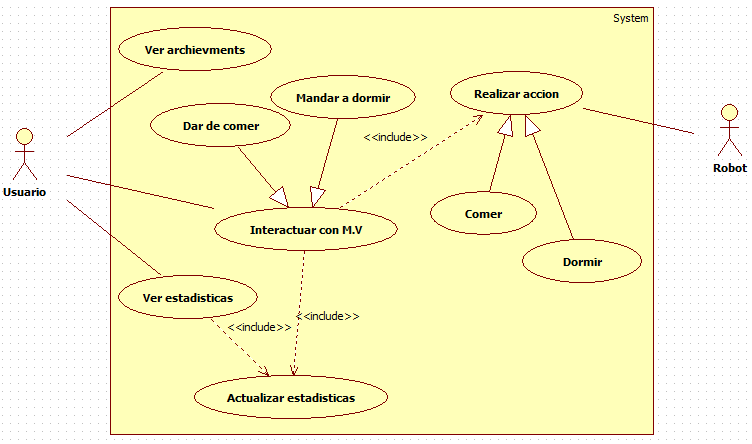
\includegraphics[scale=0.6]{caso2.png}
  \caption[~Caso de Uso Entregable 2]{Caso de Uso para el Entregable 2.}
  \label{fig:Caso2}
\end{figure}

%%
%%Caso de Uso: Actualizar estadisticas
%%
\begin{table}[htbp!]
  \centering
  \begin{tabular}{|p{4cm}|p{6cm}|}\hline
    \bf{Caso de Uso}                   & Actualizar estad\'isticas. \\ \hline
    \bf{Descripci\'on}                 & Actualiza en la base de datos las estad\'isticas de la mascota, como las veces que ha comido, hambre actual, veces que ha dormido, entre otros. \\ \hline
    \bf{Pre-condiciones}               & Mascota debe estar creada. \\ \hline
    \bf{Post-condiciones}              & Estad\'isticas actualizadas en el sistema. \\ \hline
    \bf{Requerimientos no funcionales} & -- \\ \hline
  \end{tabular}
  \caption[~Caso de Uso: Actualizar Estad\'isticas]{Caso de Uso: Actualizar Estad\'isticas.}
  \label{table:ActualizarEstadisticas}
\end{table}

%%
%%Caso de Uso: Ver Estadisticas
%%
\begin{table}[htbp!]
  \centering
  \begin{tabular}{|p{4cm}|p{6cm}|}\hline
    \bf{Caso de Uso}                   & Ver estad\'isticas. \\ \hline
    \bf{Descripci\'on}                 & Carga las estad\'isticas guardadas en la base de datos de la mascota actual y las muestra en pantalla. \\ \hline
    \bf{Pre-condiciones}               & Mascota debe estar creada. \\ \hline
    \bf{Post-condiciones}              & Se muestra en pantalla principal las estad\'isticas de la mascota actual. \\ \hline
    \bf{Requerimientos no funcionales} & Existencia de las estad\'isticas de la mascota en la base de datos. \\ \hline
  \end{tabular}
  \caption[~Caso de Uso: Ver Estad\'isticas]{Caso de Uso: Ver Estad\'isticas.}
  \label{table:VerEstadisticas}
\end{table}

%%
%%Caso de Uso: Ver Achievements
%%
\begin{table}[htbp!]
  \centering
  \begin{tabular}{|p{4cm}|p{6cm}|}\hline
    \bf{Caso de Uso}                   & Ver achievements. \\ \hline
    \bf{Descripci\'on}                 & Cargar los logros desde la base de datos, muestra los que est\'an logrados con un icono y los que no con un signo de interrogaci\'on. \\ \hline
    \bf{Pre-condiciones}               & Mascota debe estar creada. \\ \hline
    \bf{Post-condiciones}              & Se muestra en pantalla principal los logros y se puede ver su nombre, descripci\'on y si estan logrados o no. \\ \hline
    \bf{Requerimientos no funcionales} & Logros en la base de datos.  \\ \hline
  \end{tabular}
  \caption[~Caso de Uso: Ver Achievements]{Caso de Uso: Ver Achievements.}
  \label{table:VerAchievements}
\end{table}

%%
%%Caso de Uso: Dar de comer
%%
\begin{table}[htbp!]
  \centering
  \begin{tabular}{|p{4cm}|p{6cm}|}\hline
    \bf{Caso de Uso}                   & Dar de comer. \\ \hline
    \bf{Descripci\'on}                 & Detecta cuando el usuario mueve el dispositivo Android como si estuviese llenando un plato de comida vac\'io, a trav\'es de movimiento del dispositivo Android registrado por el aceler\'ometro. \\ \hline
    \bf{Pre-condiciones}               & Mascota debe estar creada. \\ \hline
    \bf{Post-condiciones}              & Alimenta a la mascota. Mascota m\'as feliz con barra de hambre m\'as vacia. Se agrega a base de datos de estad\'isticas que comi\'o una vez.   \\ \hline
    \bf{Requerimientos no funcionales} & Dispositivo Android con aceler\'ometro. \\ \hline
  \end{tabular}
  \caption[~Caso de Uso: Dar de Comer]{Caso de Uso: Dar de Comer.}
  \label{table:DarComer}
\end{table}

%%
%%Caso de Uso: Comer
%%
\begin{table}[htbp!]
  \centering
  \begin{tabular}{|p{4cm}|p{6cm}|}\hline
    \bf{Caso de Uso}                   & Comer. \\ \hline
    \bf{Descripci\'on}                 & Reacci\'on del robot al ser alimentada la mascota. \\ \hline
    \bf{Pre-condiciones}               & Usuario tiene que haberle dado de comer a la mascota. Mascota debe estar creada. \\ \hline
    \bf{Post-condiciones}              & Mascota m\'as feliz con barra de hambre m\'as vac\'ia. Se agrega a base de datos de estad\'isticas que comi\'o una vez. \\ \hline
    \bf{Requerimientos no funcionales} & Conexi\'on entre robot y dispositivo Android. \\ \hline
  \end{tabular}
  \caption[~~Caso de Uso: Comer]{Caso de Uso: Comer.}
  \label{table:Comer}
\end{table}

%%
%%Caso de Uso: Mandar a dormir
%%
\begin{table}[htbp!]
  \centering
  \begin{tabular}{|p{4cm}|p{6cm}|}\hline
    \bf{Caso de Uso}                   & Mandar a dormir. \\ \hline
    \bf{Descripci\'on}                 & Detecta cuando el usuario bloquea el sensor de proximidad del dispositivo Android, mandando a dormir a la mascota. \\ \hline
    \bf{Pre-condiciones}               & Mascota debe estar creada. \\ \hline
    \bf{Post-condiciones}              & Hace dormir a la mascota. \\ \hline
    \bf{Requerimientos no funcionales} & Dispositivo Android con sensor de proximidad. \\ \hline
  \end{tabular}
  \caption[~~Caso de Uso: Mandar a Dormir]{Caso de Uso: Mandar a Dormir.}
  \label{table:MandarDormir}
\end{table}

%%
%%Caso de Uso: Dormir
%%
\begin{table}[htbp!]
  \centering
  \begin{tabular}{|p{4cm}|p{6cm}|}\hline
    \bf{Caso de Uso}                   & Dormir. \\ \hline
    \bf{Descripci\'on}                 & Reacci\'on del robot al ser mandada a dormir la mascota. \\ \hline
    \bf{Pre-condiciones}               & Usuario tiene que haber mandado a dormir a la mascota. Mascota debe estar creada. \\ \hline
    \bf{Post-condiciones}              & Mascota m\'as feliz con barra de cansancio m\'as vac\'ia. Se agrega a base de datos de estad\'isticas que durmi\'o una vez. \\ \hline
    \bf{Requerimientos no funcionales} & Conexi\'on entre robot y dispositivo Android. \\ \hline
  \end{tabular}
  \caption[~~Caso de Uso: Dormir]{Caso de Uso: Dormir.}
  \label{table:Dormir}
\end{table}

% 
%ENTREGABLE 3
%
\newpage
\subsubsection{Entregable 3}

Los casos de uso correspondientes al Entregable 1 se detallan a continuaci\'on, desde la tabla~\ref{table:RecogerPelota} hasta la tabla~\ref{table:IrBanio}. En figura~\ref{fig:Caso3}, se muestra el diagrama de los casos de uso a implementar.

\begin{figure}[H]
  \centering
  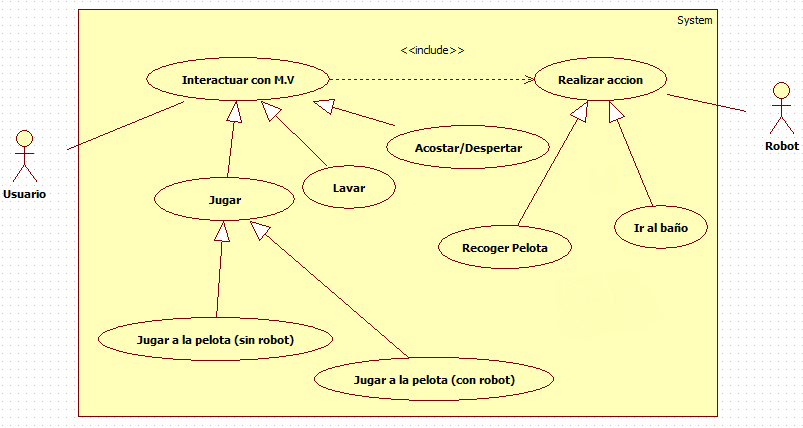
\includegraphics[scale=0.6]{caso3.png}
  \caption[~Caso de Uso Entregable 3]{Caso de Uso para el Entregable 3.}
  \label{fig:Caso3}
\end{figure}

%%
%%Caso de Uso: Recoger Pelota
%%
\begin{table}[htbp!]
  \centering
  \begin{tabular}{|p{4cm}|p{6cm}|}\hline
    \bf{Caso de Uso}                   & Recoger pelota. \\ \hline
    \bf{Descripci\'on}                 & Robot busca pelota segun color y la recoge interactuando con la aplicaci\'on confirmando que sea la pelota correcta por medio de un sensor de color. \\ \hline
    \bf{Pre-condiciones}               & Robot tiene que haber recibido instrucci\'on para recoger pelota. Mascota debe estar creada. \\ \hline
    \bf{Post-condiciones}              & Robot tiene una pelota. Informa a aplicaci\'on de exito de la operaci\'on. \\ \hline
    \bf{Requerimientos no funcionales} & Conexi\'on con robot. Dispositivo Android. Robot con los sensores apropiados. \\ \hline
  \end{tabular}
  \caption[~~Caso de Uso: Recoger Pelota]{Caso de Uso: Recoger Pelota.}
  \label{table:RecogerPelota}
\end{table}

%%
%%Caso de Uso: Jugar a la pelota (sin robot)
%%
\begin{table}[htbp!]
  \centering
  \begin{tabular}{|p{4cm}|p{6cm}|}\hline
    \bf{Caso de Uso}                   & Jugar a la pelota (sin robot). \\ \hline
    \bf{Descripci\'on}                 & Minijuego para aumentar el nivel de felicidad de la mascota. Ambientado en un juego con pelota.  \\ \hline
    \bf{Pre-condiciones}               & Mascota debe estar creada.  \\ \hline
    \bf{Post-condiciones}              & Los niveles apropiados son actualizados (felicidad, energ\'ia, etc). Se agrega a base de datos que jug\'o una vez.  \\ \hline
    \bf{Requerimientos no funcionales} & -- \\ \hline
  \end{tabular}
  \caption[~~Caso de Uso: Jugar a la Pelota (Sin Robot)]{Caso de Uso: Jugar a la Pelota (Sin Robot).}
  \label{table:JugarPelota-SR}
\end{table}

%%
%%Caso de Uso: Jugar a la pelota (con robot)
%%
\begin{table}[htbp!]
  \centering
  \begin{tabular}{|p{4cm}|p{6cm}|}\hline
    \bf{Caso de Uso}                   & Jugar a la pelota (con robot). \\ \hline
    \bf{Descripci\'on}                 & Minijuego para aumentar el nivel de felicidad de la mascota. Ambientado en un juego con pelota. Este interactua con el robot solicitando al usuario buscar una pelota de un color especifico. \\ \hline
    \bf{Pre-condiciones}               & Mascota debe estar creada, conexi\'on con el robot, una cantidad de energ\'ia m\'inima. \\ \hline
    \bf{Post-condiciones}              & Los niveles apropiados son actualizados (felicidad, energ\'ia, etc). Se agrega a base de datos que jug\'o una vez.  \\ \hline
    \bf{Requerimientos no funcionales} & Dispositivo Android. Robot con los sensores apropiados. \\ \hline
  \end{tabular}
  \caption[~~Caso de Uso: Jugar a la Pelota (Con Robot)]{Caso de Uso: Jugar a la Pelota (Con Robot).}
  \label{table:JugarPelota-CR}
\end{table}

%%
%%Caso de Uso: Lavar
%%
\begin{table}[htbp!]
  \centering
  \begin{tabular}{|p{4cm}|p{6cm}|}\hline
    \bf{Caso de Uso}                   & Lavar.\\ \hline
    \bf{Descripci\'on}                 & Detecta cuando el usuario mueve el dispositivo android como si estuviese lavando a la mascota, a trav\'es de movimiento del dispositivo android registrado por el aceler\'ometro. Si se esta conectado al robot genera una reacci\'on en el. \\ \hline
    \bf{Pre-condiciones}               & Mascota debe estar creada. \\ \hline
    \bf{Post-condiciones}              & Limpia desechos , actualizar estado de salud en la base de datos.  \\ \hline
    \bf{Requerimientos no funcionales} & Dispositivo Android con aceler\'ometro. \\ \hline
  \end{tabular}
  \caption[~~Caso de Uso: Lavar]{Caso de Uso: Lavar.}
  \label{table:Lavar}
\end{table}

%%
%%Caso de Uso: Limpiar
%%
\begin{table}[htbp!]
  \centering
  \begin{tabular}{|p{4cm}|p{6cm}|}\hline
    \bf{Caso de Uso}                   & Limpiar. \\ \hline
    \bf{Descripci\'on}                 & El usuario limpia los desechos dejado por la mascota. \\ \hline
    \bf{Pre-condiciones}               & Mascota debe estar creada, que existan desechos. \\ \hline
    \bf{Post-condiciones}              & Mascota m\'as feliz con barra de salud m\'as llena, se agrega a base de dato de estad\'isticas que fue limpiado una vez por cada desecho eliminado. \\ \hline
    \bf{Requerimientos no funcionales} & Conexi\'on entre robot y dispositivo Android. \\ \hline
  \end{tabular}
  \caption[~~Caso de Uso: Ir al Ba\~no]{Caso de Uso: Ir al Ba\~no.}
  \label{table:IrBanio}
\end{table}

%
%ENTREGABLE 4
%
\newpage
\subsubsection{Entregable 4}

Los casos de uso correspondientes al Entregable 1 se detallan a continuaci\'on, desde la tabla~\ref{table:Sacudirse} hasta la tabla~\ref{table:SacarPulgas}. En figura~\ref{fig:Caso4}, se muestra el diagrama de los casos de uso a implementar.

\begin{figure}[H]
  \centering
  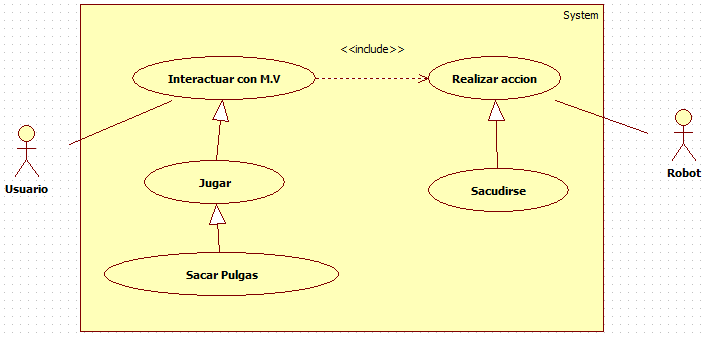
\includegraphics[scale=0.6]{caso4.png}
  \caption[~Caso de Uso Entregable 4]{Caso de Uso para el Entregable 4.}
  \label{fig:Caso4}
\end{figure}

%%
%%Caso de Uso: Sacudirse
%%
\begin{table}[htbp!]
  \centering
  \begin{tabular}{|p{4cm}|p{6cm}|}\hline
    \bf{Caso de Uso}                   & Sacudirse. \\ \hline
    \bf{Descripci\'on}                 & Reacci\'on del robot al sacar pulgas. \\ \hline
    \bf{Pre-condiciones}               & Mascota debe estar creada. Robot recibi\'o instrucci\'on para sacudirse. \\ \hline
    \bf{Post-condiciones}              & Robot se sacude. \\ \hline
    \bf{Requerimientos no funcionales} & Conexi\'on con robot. Dispositivo Android. \\ \hline
  \end{tabular}
  \caption[~~Caso de Uso: Sacudirse]{Caso de Uso: Sacudirse.}
  \label{table:Sacudirse}
\end{table}

%%
%%Caso de Uso: Sacar pulgas
%%
\begin{table}[htbp!]
  \centering
  \begin{tabular}{|p{4cm}|p{6cm}|}\hline
    \bf{Caso de Uso}                   & Sacar pulgas. \\ \hline
    \bf{Descripci\'on}                 & Minijuego ambientado en el acto de sacar pulgas a una mascota. En caso de estar conectado a un robot genera reacci\'on en el. \\ \hline
    \bf{Pre-condiciones}               & Mascota creada, mascota debe tener un minimo de energia. \\ \hline
    \bf{Post-condiciones}              & Mascota m\'as feliz. Se almacena en la base de datos que la mascota jug\'o. \\ \hline
    \bf{Requerimientos no funcionales} & Dispositivo Android.  \\ \hline
  \end{tabular}
  \caption[~~Caso de Uso: Sacar Pulgas]{Caso de Uso: Sacar Pulgas.}
  \label{table:SacarPulgas}
\end{table}

\newpage
%
%Item 5.3
%
\section{Plan de mantenci\'on}
Phyrex asegura soluciones efectivas a la brevedad de posibles errores surgidos en la aplicaci\'on. Ser\'a posible reportar estos errores mediante website, redes sociales (Facebook, Twitter, Google+) en primera instancia. Tambi\'en Google Play se presenta como opci\'on una vez se realice el lanzamiento en esta plataforma.

Una vez conocidos los posibles problemas, se proceder\'a a realizar una verificaci\'on del error, y publicaci\'on de nuevas releases con la soluci\'on implementada. Se priorizar\'an requerimientos esenciales acordados con cliente y problemas de compatibilidad con dispositivos que cumplan los requisitos ya expuestos.

Phyrex no se responsabiliza por da\~nos o problemas causados por armado incorrecto de LEGO Mindstorms NXT o mal uso de la aplicaci\'on, sin embargo, se compromete a entregar servicios de asistencia y atenci\'on al cliente en armado del robot, instalaci\'on de la aplicaci\'on y uso de \'esta.

\newpage
